\documentclass[a4paper,12pt]{article}
\usepackage[utf8]{inputenc}
\usepackage{fancyhdr}
\usepackage{enumitem}
\usepackage{hyperref}
\usepackage{natbib}
\usepackage[french]{babel}

\setlength{\parindent}{1cm}
\usepackage{mwe,lipsum}
\usepackage[section]{placeins}
\usepackage{dblfloatfix}
\usepackage{float}
\usepackage[utf8]{inputenc}
\usepackage[T1]{fontenc}
\usepackage{graphicx}
\usepackage{fullpage}
\usepackage{eso-pic}
\usepackage{layout}
\usepackage{indentfirst}
\usepackage{siunitx}
\usepackage{amsmath}
\usepackage{amssymb}
\usepackage{tabularx}
\usepackage{multicol}
\usepackage{multirow}

\usepackage{caption}
\usepackage{subcaption}

\setlength{\headsep}{0.3cm}
\renewcommand*\contentsname{Table des matières}

\begin{document}
	\pagestyle{fancy}
	\headheight=15pt
	\fancyhf{}
	\renewcommand{\footrulewidth}{0.4pt}
	
	\lhead{DNS over HTTPS}
	\rhead{IP}
	% \lfoot{Equipe 9 - 2020}
	\rfoot{\thepage}
	
	%   TITLE PAGE
	\begin{titlepage}
		
		\begin{center}
			\rule{\textwidth}{1pt} % Thick horizontal rule
			
			\vspace{2pt}\vspace{-\baselineskip} % White space between rules
			
			\rule{\textwidth}{0.4pt} % Thin horizontal rule
			
			\vspace{0.1\textheight} % White space between the top rules and title
			
			%------------------------------------------------
			%	Title
			%------------------------------------------------
			
			\textcolor{black} {
				{\Huge DNS over HTTPS}\\[0.5\baselineskip]
			}
			
			\vspace{0.01\textheight} % White space between the title and short horizontal rule
			
			\rule{0.3\textwidth}{0.4pt} % Short horizontal rule under the title
			
			\vspace{0.1\textheight}
			
			%------------------------------------------------
			%	Author
			%------------------------------------------------
			
			{\Large \textsc{Arnaud Lombardi - Théo Grosperrin}} % Author name
			
			\vspace{0.025\textheight}
			
			{\large \textsc{\today}}
			
			\vfill % White space between the author name and publisher
			
		\end{center}
		
		%------------------------------------------------
		%	Publisher
		%------------------------------------------------
		
		\centering
		{
\includegraphics[scale=0.5]{Images/INSA_LOGO.png}}\\[1.7\baselineskip]
		{
\includegraphics[scale=0.18]{Images/TC.jpg}}
		
		\vspace{0.1\textheight} % White space under the publisher text
		
		%------------------------------------------------
		%	Bottom rules
		%------------------------------------------------
		
		\centering
		
		\rule{\textwidth}{0.4pt} % Thin horizontal rule
		
		\vspace{2pt}\vspace{-\baselineskip} % White space between rules
		
		\rule{\textwidth}{1pt} % Thick horizontal rule
		
	\end{titlepage}
	
	% Front matter %
	\setcounter{page}{1}
	\pagenumbering{arabic}
	
	%------------------------------------------------
	%	Table of contents
	%------------------------------------------------
	\hspace{2cm}
	\tableofcontents
	
	\newpage
	
	\section{En quelques mots, qu'est que le DoH ?}
	Il s'agit de la résolution des requêtes DNS en utilisant le protocole HTTPS, au lieu de simples requêtes en clair sur le port 53 (DNS classique). L'objectif de cette méthode est d'augmenter la sécurité du cote utilisateur : cela permet d'améliorer la vie privée de l'utilisateur (le trafic entre le client et le serveur DNS est chiffré, illisible par les machines se trouvant sur le chemin), et d'éviter les attaques de type "man-in-the-middle".
	
	\section{Détails techniques}
	Le DoH est un standard publié par l'IETF : \href{https://tools.ietf.org/html/rfc8484}{RFC 8484}.
	
	\subsection{Le fonctionnement du DNS et ses limites}
	DNS est un acronyme qui signifie « Domain Name System » et peut se traduire par « système de noms de domaine ».
	Le DNS est un service permettant de faire le lien entre les noms de domaines et les adresses IP qui leurs sont associées (ex : google.fr = 216.58.198.195).
	Pour cela DNS a besoin de plusieurs serveurs pour répondre au requête DNS. 
	Les applications vont passer par un serveur DNS mandataire qui contactera dans un premier temps l'un des 13 serveurs racine aléatoirement en lui demandant les informations sur le nom de domaine (Adresse IP ,SPF ,DKIM ... ). De manière récursif, le serveur mandataire obtient les instructions concernant les adresses des prochains NS (Name Server), jusqu'à obtenir la réponse d'un serveur faisant autorité. Il existe un cas ou l'application va elle même récupère les informations de manière récursive.
	
	\begin{figure}[H]
		\begin{center}
			{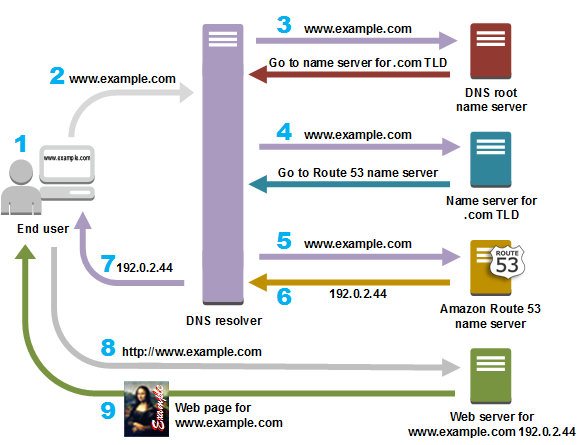
\includegraphics[scale=0.5]{Images/routes-traffic.png}}
		\end{center}
		\caption{Schéma d'une requête DNS.[1]}		 
		
	\end{figure}
	\lfoot{[1] https://www.seomining.com/website-deployment/module3/registering-domain-names.php}
	
	Une demande DNS consiste à envoyer sur le port 53 du serveur une requête en clair pour récupérer l'information sur le nom de domaine voulu en passant par les diffèrents serveur .
	
	Limite :
	DNS utilise en général UDP et le port 53. La taille maximale des paquets utilisée est de 512 octets. Si une réponse dépasse cette taille, la norme prévoit que la requête doit être renvoyée sur le port TCP 53. Ce cas est cependant rare et évité, et les firewalls bloquent souvent le port TCP 53.
	
	Plusieurs failles de DNS sont connus dû au fait que les requêtes soit envoyer en clair : 
	Une des failles mises en avant est la possibilité d'intercepter les paquets transmis. 
	Les serveurs DNS communiquent au moyen de paquets uniques et non signés. 
	Ces deux spécificités rendent l'interception très aisée. 
	L'interception peut se concrétiser de différentes manières, notamment via une attaque de type « man in the middle », de l'écoute des données transférées et de l'envoi de réponse falsifiée.
	Les paquets des serveurs DNS étant faiblement sécurisés, authentifiés par un numéro de requête, il est possible de fabriquer de faux paquets.
	Par exemple, un utilisateur qui souhaite accéder au site http://mabanque.example.com fait une demande au site DNS.
	Il suffit, à ce moment, qu'un attaquant réponde à la requête de l'utilisateur avant le serveur DNS pour que l'utilisateur se retrouve sur un site d'hameçonnage.
	La trahison par un serveur, ou corruption de données, est, techniquement, identique à une interception des paquets.
	La seule différence venant du fait que l'utilisateur envoie volontairement sa requête au serveur. 
	
	Cette situation peut arriver lorsque, par exemple, l'opérateur du serveur DNS souhaite mettre en avant un partenaire commercial.
	L'empoisonnement du cache DNS ou pollution de cache DNS (en anglais, DNS cache poisoning) est une technique permettant de leurrer les serveurs DNS afin de leur faire croire qu'ils reçoivent une requête valide tandis qu'elle est frauduleuse.
	Une attaque par déni de service (ou attaque par saturation; en anglais, Denial of Service attack ou DoS attack) est une attaque sur un serveur informatique qui résulte en l'incapacité pour le serveur de répondre aux requêtes de ses clients.
	DoH permet de se prémunir de toute attaque impliquant un tiers, de l’homme du milieu aux middleboxes car il utilise le port 443 (HTTPS) utilisé pour les connexions sécurisée et qui permet l'assurance de l'origine de la réponse et de sa non-altération.
	
	\subsection{Le fonctionnement du DoH}
	Cette solution est récente, ayant fait l’objet d’une standardisation par l’IETF (Internet Engineering Task Force) en octobre 2018 (RFC 8484).  Le mécanisme décrit comment les requêtes et réponses sont chiffrées, encapsulées dans un flux HTTPS.
	Un serveur prenant en charge ce protocole est appelé «serveur DoH» pour
	le différencier d'un "serveur DNS" ecoutant sur le port 443 (HTTPS). 
	De même, un client qui prend en charge ce protocole est appelé un "client DoH".
	Le client DoH est configuré avec un modèle URI [ RFC6570 ], qui
	décrit comment construire l'URL à utiliser pour la résolution.
	Un client DoH utilise la configuration pour sélectionner un URI, et donc le serveur DoH, qui doit être utilisé pour la résolution. La [ RFC2818 ] définit comment	HTTPS vérifie l'identité du serveur DoH.
	Un client DoH en-capsule une seule requête DNS dans une requête HTTP à l'aide de 
	la méthode HTTP GET ou POST.
	\begin{figure}[H]
		\begin{center}
			{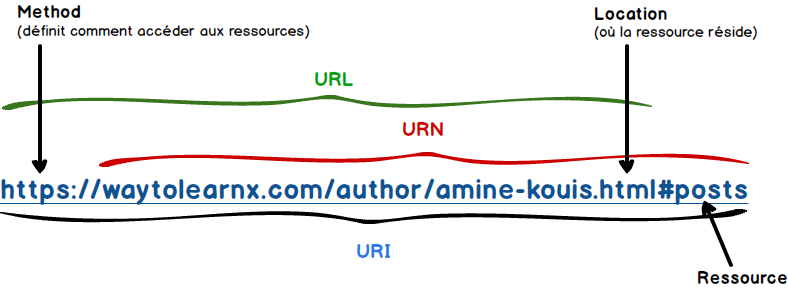
\includegraphics[scale=0.5]{Images/difference-entre-uri-et-url.png}}
		\end{center}
		\caption{Modèle d'un URI.[2]}		 
		
	\end{figure}
	\lfoot{[2] https://waytolearnx.com/2018/09/difference-entre-uri-et-url.html}
	DoH utilisent donc le modèle URI  "https://dnsserver.example.net/dns-query{?dns}" pour effectuer la résolution des différents nom de domaine. 
	\begin{figure}[H]
		\begin{center}
			{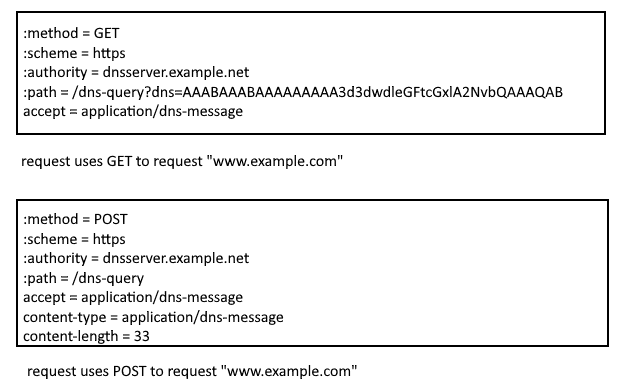
\includegraphics[scale=0.5]{Images/requetedoh.png}}
		\end{center}
		\caption{Requête DOH POST et GET.[3]}		 
		
	\end{figure}
	\lfoot{[3] https://tools.ietf.org/html/rfc8484}
	Le serveur reçoit cette requête puis effectue les requête DNS nécessaire pour effectuer la résolution de nom et réponds au client la correspondance entre le nom de domaine et son adresse IP.
	
	
	\section{Les différentes implémentations typiques}
	
	\subsubsection{DoH natif au sein du navigateur}
	
	\begin{figure}[H]
		\begin{center}
			{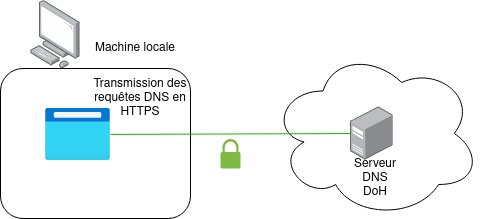
\includegraphics[scale=0.6]{Images/schema_doh_native.png}}
		\end{center}
		\caption{Schéma de l'implémentation native de DoH au sein d'une application.}
	\end{figure}

	Son principe est le suivant : la routine d'exécution de la requête DNS habituellement exécutée par le système d'exploitation est outrepassée par le navigateur qui implémente sa propre routine : celle qui utilise le DNS over HTTPS. Ainsi, la transition entre DNS classique et DoH est invisible aux yeux du système d'exploitation. 
	
	Cela permet d'utiliser ce nouveau protocole sans dépendre de l'implémentation au niveau de l'OS. C'est la méthode qui est utilisée actuellement par Google Chrome et Mozilla Firefox.
	
	Afin d'envoyer une requête au serveur DoH, le navigateur initie une session TLS avec le serveur, puis  effectue une requête HTTP de type GET indiquant le nom de domaine a résoudre, ainsi que le type de champ souhaité.
	
	Par exemple, imaginons que l'on cherche à trouver l'adresse IPv4 associée à twitter.com, en passant par le serveur DNS over HTTPS de Google.
	L'application effectue donc une requête GET vers \url{https://8.8.8.8/resolve?name=twitter.com&type=A}.
	
	La syntaxe est identique à celle d'une API.
	
	\newpage
	
	L'échange se déroule ainsi :
	\begin{figure}[H]
		\begin{center}
			{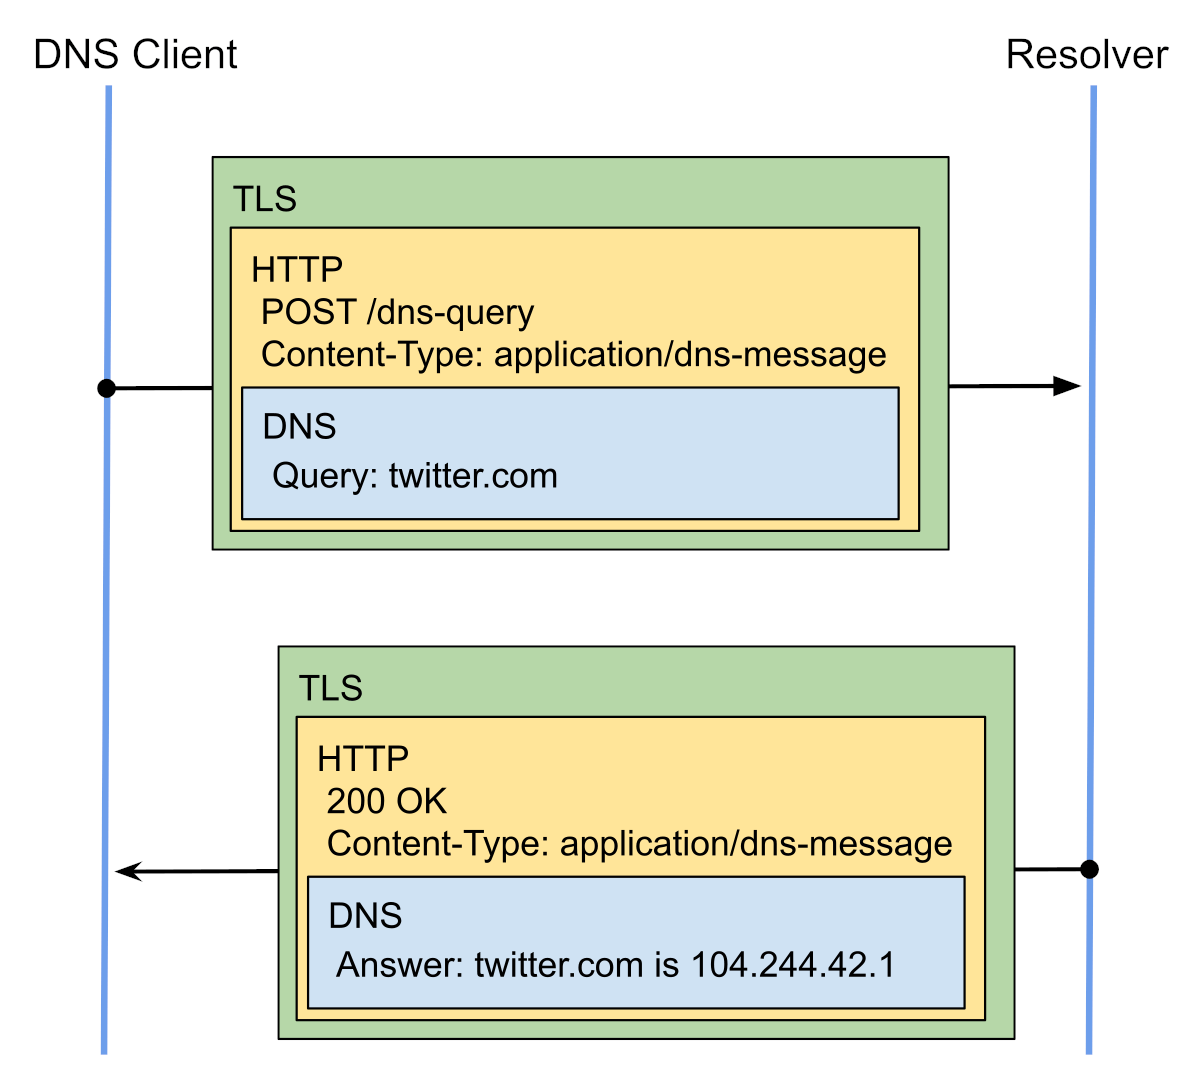
\includegraphics[scale=0.2]{Images/tls-example.png}}
		\end{center}
		\caption{Schéma des échanges lors d'une requête DoH.}
	\end{figure}
	
	Le serveur renvoie des données au format JSON contenant l'adresse IPv4 de twitter.com.
	
	\begin{figure}[H]
		\begin{center}
			{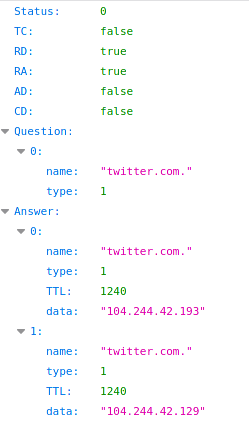
\includegraphics[scale=0.6]{Images/out_json.png}}
		\end{center}
		\caption{Réponse du serveur a la requête GET.}
	\end{figure}
	
	
 	\begin{figure}[H]
	 	\begin{center}
	 		{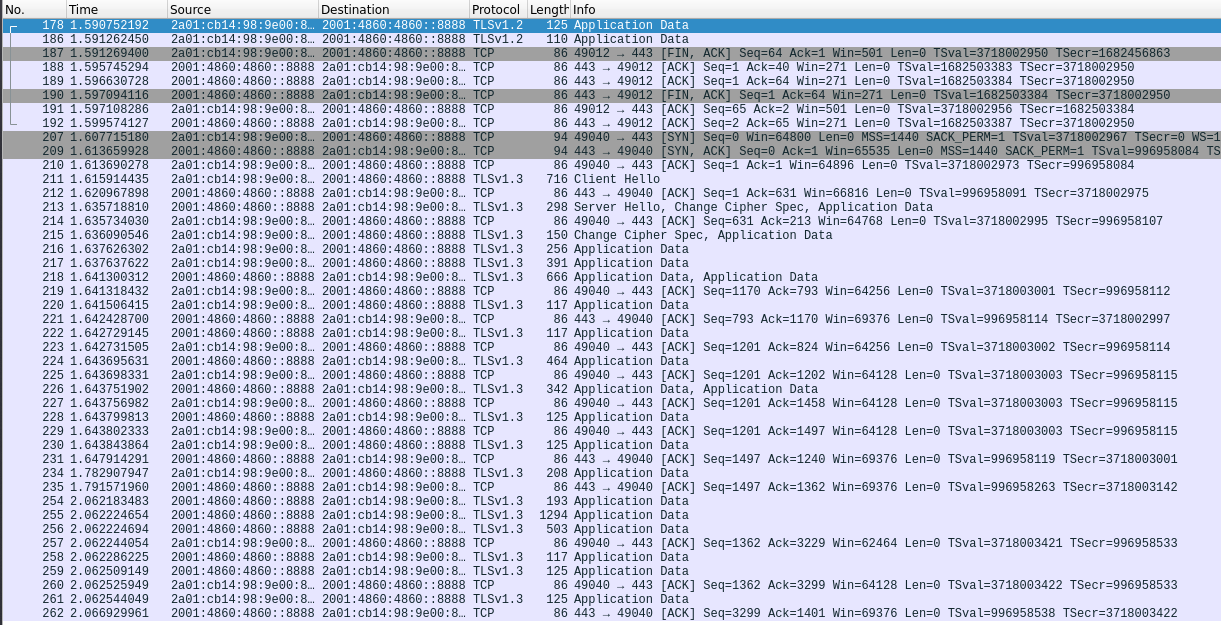
\includegraphics[scale=0.55]{Images/doh-wireshark.png}}
	 	\end{center}
	 	\caption{Capture Wireshark de l'échange DoH.}
	\end{figure}

	D'un point de vue externe, impossible de voir qu'il s'agit de trafic DNS, tout ce que l'on voit, c'est un handshake TLS entre le serveur et le client, puis des données chiffrées. Étant donné que n'importe quel type de données peuvent se trouver dans un échange chiffré, cela peut poser problème dans un environnement d'entreprise par exemple : l'adresse du serveur DoH cible dépend entièrement de l'application et de ses éventuels paramètres (le paramètre global du système d'exploitation n'est pas pris en compte, l'administrateur système perd donc la main sur ce paramètre). 
	
	Le filtrage et certains contrôles s'effectuent sur la base du DNS (exemple : filtrage des adresses non pertinentes pour le travail, ou bien encore filtrage sur une liste contenant des adresses dangereuses, pouvant potentiellement infecter les postes de l'entreprises). 
	
	Cette méthode offre donc un moyen facile de contourner les filtrages DNS mis en place par l'administrateur système, ce qui n'est pas l'objectif recherché...
	
	\subsubsection{Proxy DoH sur le réseau local}
	
	Dans ce scénario, les machines du réseau local effectuent des requêtes DNS traditionnelles sur le port 53, vers un serveur DNS installé sur le réseau local. Ce serveur DNS effectue ensuite une requête DNS récursive vers un resolver DoH. Ainsi, la requête est masquée lorsqu'elle sort du LAN.
	
	\begin{figure}[H]
		\begin{center}
			{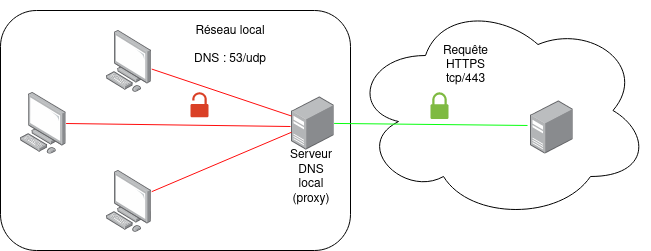
\includegraphics[scale=0.6]{Images/schema_doh_proxy_lan.png}}
		\end{center}
		\caption{Schéma de l'implémentation d'un serveur DoH proxy sur un réseau local.}
	\end{figure}
	
	On constate bien l'inconvénient de ce système : les requêtes entre les clients et le serveur local ne sont pas sécurisées, et on se base sur le fait que l'on fait confiance au serveur proxy (qui lui même fait confiance aveuglément au resolver DoH)
	Cependant, il s'agit d'un méthode d'implémentation relativement facile à mettre en place, puisqu'elle n'implique que peu de modifications sur le réseau existant, simplement l'ajout d'un proxy sur le LAN.
	Cette méthode permet donc de conserver le filtrage DNS mis en place dans le cas d'une entreprise, pour peu que le DoH soit désactivé sur les applications des postes utilisateurs.
	
	\subsubsection{Proxy DoH sur système local}
	
	Ici, le système est configuré pour envoyer les requêtes DNS à lui-même, puisqu'on installe un serveur proxy sur celui-ci. Ce proxy se charge d'effectuer les requêtes de manière sécurisée (donc DoH) pour chaque requête DNS classique qu'il reçoit.
	Cette méthode permet de forcer l'utilisation du DoH sur système d'exploitation ne l'implémentant pas et sur des applications ne l'implémentant pas également, sans pour autant devoir faire appel a une machine extérieure (comme dans le cas du proxy DoH sur LAN).
	Cependant, cette methode est lourde 
	Cette méthode permet d'utiliser des applications n'implémentant pas le DoH de manière native sans compromettre la sécurité des requêtes sur le LAN. Cependant, elle est lourde puisqu'elle implique d'installer un proxy sur chaque machine.
	
	\begin{figure}[H]
		\begin{center}
			{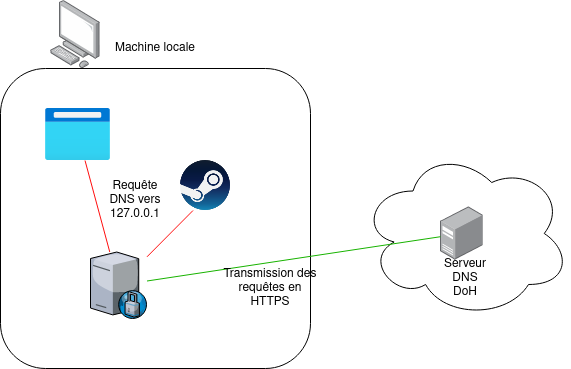
\includegraphics[scale=0.6]{Images/schema_doh_proxy_local.png}}
		\end{center}
		\caption{Schéma de l'implémentation d'un serveur proxy DoH sur le système local.}
	\end{figure}

	\section{Mise en contexte}
	
	\subsection{Support logiciel}
	
	\subsubsection{Système d'exploitation}
	DoH est implémenté sur Windows 10 depuis la version 19628 (mai 2020), iOS 14 et macOS 11 depuis fin 2020. Le support est donc très récent (et donc restreint).
	\subsubsection{Navigateurs compatibles}
	Les navigateurs les plus populaires sont compatibles DoH :
	\begin{itemize}
		\item Mozilla Firefox : suite à un partenariat avec Cloudflare, l'option est disponible des 2018. Depuis le 25 février 2020, Firefox active le DoH par défaut pour tous les utilisateurs des Etats-Unis.
		\item Google Chrome : disponible depuis la version 83 pour Windows et macOS, la fonctionnalité est accessible depuis les paramètres du navigateur. En septembre 2020, la version Android du navigateur supporte le DoH.
		\item Microsoft Edge : compatible (le navigateur est un fork de Google Chrome).
	\end{itemize}
	\subsubsection{Serveurs compatibles}
	BIND 9, un serveur DNS open-source et très répandu, a introduit le support du DoH en février 2021, sur la version 9.17.10.
	Quant à Unbound, il le supporte depuis octobre 2020 (version 1.12.0). Il supportait déjà le DoT (DNS over TLS) depuis décembre 2011.
	\subsection{Critiques}
	Le DoH, comme de nombreuses technologies cherchant a améliorer la sécurité, n'a pas manqué d'être le sujet de critiques diverses. En effet, certains pirates ont su tirer profit de ce protocole : en 2019, le ver Godlua, qui a servi à exécuter diverses attaques de type DDoS, a utilisé le DoH afin de masquer la destination de son serveur de contrôle.
	Mais il a également été critiqué par le gouvernement du Royaume-Uni : le pays a mis en place divers filtres afin de bloquer des sites web proposant du contenu illégalement, ou bien l'accès au sites pornographiques (pour lesquels il faut entrer un numéro de carte bancaire afin de prouver la majorité du visiteur dans ce pays). Mozilla a été accusé de "Internet Villain" par l'ISPA (Internet Service Providers Association) pour avoir sapé les standards en matière de sécurité web du Royaume-Uni. Mozilla a été contraint de désactiver par défaut le DoH sur son navigateur pour les utilisateurs anglo-saxons.\href{https://www.theguardian.com/technology/2019/sep/24/firefox-no-uk-plans-to-make-encrypted-browser-tool-its-default}{Source}
	\section{Les problèmes que peuvent poser le DoH}	
	DoH peut poser des problèmes de vie privé car HTTP est bavard, très bavard. Ainsi, une requête DNS contient très peu d'informations sur le client, alors que HTTP transmet plein d'informations inutiles et dangereuses comme Accept-Language: ou User-Agent:, qui peuvent servir à identifier un utilisateur. Sans compter bien sûr les cookies (RFC 6265). Il s'agit là d'un vrai problème. Des solutions ont été proposées (cf. l'\href{https://en.wikipedia.org/wiki/Internet_Draft}{Internet-Draft} \href{https://datatracker.ietf.org/doc/draft-dickinson-doh-dohpe/}{draft-dickinson-doh-dohpe}) mais n'ont guère suscité d'intérêt.
	On peut aussi souligner le fait que le DoH n'est pas propre d'un point de vue technique car sur internet une application est censé tourner sur SCTP,TCP ou bien UDP mais pas sur du HTTPS.
	D'autres problème se posent mais ne concerne pas que le DoH comme le fait d'empêcher (rendre plus difficile) la censure (DoT a ce même problème ) ou alors la centralisation d'internet en effectuent des requêtes sur les serveurs des GAFA
    ( Les résolveurs DNS publics, comme Google Public DNS posent le même problème.) la solution à ce problème serais de multiplier les serveurs DoH.
\end{document}